\documentclass[a4paper, fleqn]{article}

\usepackage{amsmath}
\usepackage{enumitem}
\usepackage{graphicx}

\begin{document}

\title{Homework I \\ Introduction to Physical Chemistry}
\author{Basil R. Yap 1001690}
\date{2018 January 25}
\maketitle

\section{Question 1}
\begin{enumerate}[label=(\alph{*})]
\item 310.95 K
\item -176.15 $^\circ$C
\item 8720 nm
\item $0.173\text{\AA}\times(10^{-10})^3=1.73\times10^{-31}\text{ m}^3$
\item $\frac{1.76\times10^{-19}\text{ J}}{1.602\times10^{-19}}=1.10\text{ eV}$
\item $3.1 \text{ mols}\times6.022\times10^{23}=1.87\times10^{24}$
\end{enumerate}

\section{Question 2}
\begin{enumerate}[label=(\alph{*})]
\item Cl(Z=17): $1s^2,2s^2,2p^6,3s^2,3p^5$
\item Cu(Z=29): $1s^2,2s^2,2p^6,3s^2,3p^6,4s^1,3d^{10}$
\item Cu$^{+2}$(Z=29): $1s^2,2s^2,2p^6,3s^2,3p^6,4s^2,3d^7$
\end{enumerate}

\pagebreak

\section{Question 3}
\begin{enumerate}[label=(\alph{*})]
\item $\lambda=640$nm\\
$\begin{aligned}v&=\frac{c}{\lambda}\\&=\frac{3.00\times10^{17}}{640}\\&=4.69\times10^{14}\text{s}^{-1}\end{aligned}$
\item Visible light
\item $\begin{aligned}E&=hv\\&=6.626\times10^{-34}\times4.69\times10^{14}\\&=3.11\times10^{-19}\text{ J}\end{aligned}$
\item \begin{itemize}
\item A: Constructive
\item B: Destructive
\item C: Constructive
\end{itemize}
\end{enumerate}

\pagebreak

\section{Question 4}
\begin{enumerate}[label=(\alph{*})]
\item Figure 1\\
\begin{figure}[h!]
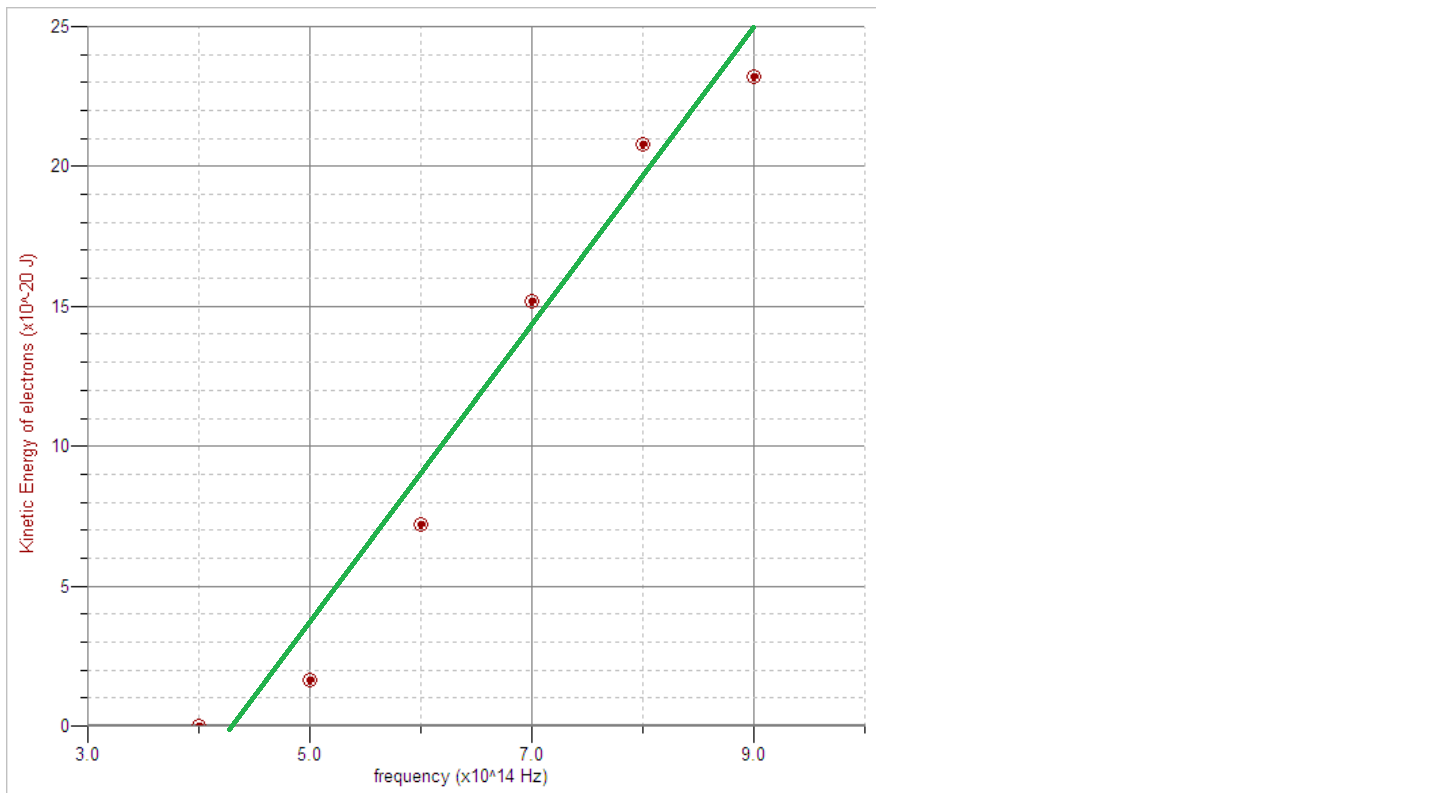
\includegraphics[width=\linewidth]{assets/201801310030.png}
\caption{Best-fit line}
\label{fig:graph1}
\end{figure}

\item $\begin{aligned}h&=\frac{\Delta KE}{\Delta f}\\&=\frac{25.0\times10^{-20}-9.0\times10^{-20}}{9.0\times10^{14}-6.0\times10^{14}}\\&=5.33\times10^{-34}\text{ Js}\end{aligned}$
\item Threshold frequency is \textit{approximately} $4.2\times10^{14}$ Hz
\item \begin{enumerate}
\item[i)] The kinetic energy of the emitted electron is \textit{approximately} $14.2\times10^{-20}$ J
\item[ii)] $\begin{aligned}KE&=\frac{1}{2}mv^2\\14.2\times10^{-20}&=\frac{1}{2}(9.1\times10^{-31})v^2\\v^2&=3.12\times10^{11}\\v&=5.59\times10^5\text{ ms}^{-1}\end{aligned}$
\item[iii)] $\begin{aligned}\lambda&=\frac{h}{mv}\\&=\frac{6.626\times10^{-34}}{9.1\times10^{-31}\times5.59\times10^5}\\&=1.30\times10^{-9}\text{ m}\end{aligned}$
\item[iv)] $\begin{aligned}E&=eV\\14.2\times10^{-20}&=(-1.6\times10^{-19})V\\V&=-0.89\text{ V}\end{aligned}$
\end{enumerate}
\end{enumerate}

\pagebreak

\section{Question 5}
\begin{enumerate}[label=(\alph{*})]
\item $\begin{aligned}E&=hv\\&=6.626\times10^{-34}\times1.52\times10^{13}\\&=1.01\times10^{-20}\text{ J}\end{aligned}$
\item Considering at threshold,\\
$\begin{aligned}E&=hv_0\\1.03\times10^{-20}&=(6.626\times10^{-34})v_0\\v_0&=1.55\times10^{13}\text{ Hz}\end{aligned}$
\item $\begin{aligned}E&=\phi+KE\\E&=hv+KE\\1.01\times10^{-20}&=(6.626\times10^{-34})(8.95\times10^{12})+KE\\KE&=1.01\times10^{-20}-5.93\times10^{-21}\\&=4.17\times10^{-21}\text{ J}\end{aligned}$
\item $\begin{aligned}KE&=\frac{1}{2}mv^2\\4.17\times10^{-21}&=\frac{1}{2}(9.1\times10^{-31})v^2\\v^2&=9.16\times10^9\\v&=9.57\times10^4\text{ms}^{-1}\end{aligned}$
\end{enumerate}

\pagebreak

\section{Question 6}
\begin{enumerate}[label=(\alph{*})]
\item Consider the maximum wavelength where an electron would be ejected,\\
$\begin{aligned}\lambda&=\frac{hc}{E}\\&=\frac{(6.626\times10^{-34})(3.00\times10^8)}{2.52\times1.602\times10^{-19}}\\&=4.92\times10^{-7}\\&=492\text{ nm}\end{aligned}$\\
The incoming wavelength is higher than the threshold wavelength, electrons will be ejected from the metal.\\
$\begin{aligned}E&=\frac{hc}{\lambda}\\&=\frac{(6.626\times10^{-34})(3.0\times10^8)}{550\times10^{-9}}\\&=3.61\times10^{-19}\\n&=\frac{10\times10^{-3}}{E}\\&=\frac{10\times10^{-3}}{3.61\times10^{-19}}\\&=2.77\times10^{16}\text{s}^{-1}\end{aligned}$
\item The incoming wavelength is lower than the threshold wavelength, no electrons will be ejected from the metal.
\end{enumerate}

\end{document}